% Module architecture of the SySO automation project for the README.
% Layers follow the thesis diagram (docs/thesis/images/marcopractico/planificacion/
% arquitectura_modulos.tex); colored solid modules are MVP scope, gray dashed
% modules belong to the full project vision.
%
% Build (from this directory):
%   pdflatex -jobname=architecture-light architecture.tex
%   pdflatex -jobname=architecture-dark "\def\DARKMODE{1}% Module architecture of the SySO automation project for the README.
% Layers follow the thesis diagram (docs/thesis/images/marcopractico/planificacion/
% arquitectura_modulos.tex); colored solid modules are MVP scope, gray dashed
% modules belong to the full project vision.
%
% Build (from this directory):
%   pdflatex -jobname=architecture-light architecture.tex
%   pdflatex -jobname=architecture-dark "\def\DARKMODE{1}% Module architecture of the SySO automation project for the README.
% Layers follow the thesis diagram (docs/thesis/images/marcopractico/planificacion/
% arquitectura_modulos.tex); colored solid modules are MVP scope, gray dashed
% modules belong to the full project vision.
%
% Build (from this directory):
%   pdflatex -jobname=architecture-light architecture.tex
%   pdflatex -jobname=architecture-dark "\def\DARKMODE{1}% Module architecture of the SySO automation project for the README.
% Layers follow the thesis diagram (docs/thesis/images/marcopractico/planificacion/
% arquitectura_modulos.tex); colored solid modules are MVP scope, gray dashed
% modules belong to the full project vision.
%
% Build (from this directory):
%   pdflatex -jobname=architecture-light architecture.tex
%   pdflatex -jobname=architecture-dark "\def\DARKMODE{1}\input{architecture.tex}"
%   pdftocairo -png -transp -singlefile -r 200 architecture-light.pdf architecture-light
%   pdftocairo -png -transp -singlefile -r 200 architecture-dark.pdf architecture-dark
\documentclass[tikz,border=14pt]{standalone}
\usepackage[T1]{fontenc}
\usepackage{helvet}
\renewcommand{\familydefault}{\sfdefault}
\usetikzlibrary{positioning}

\ifdefined\DARKMODE
  % GitHub dark palette
  \definecolor{fgText}{HTML}{E6EDF3}
  \definecolor{fgMuted}{HTML}{9198A1}
  \definecolor{mgmtFill}{HTML}{0D2540}\definecolor{mgmtLine}{HTML}{4493F8}
  \definecolor{inFill}{HTML}{12261E}\definecolor{inLine}{HTML}{3FB950}
  \definecolor{procFill}{HTML}{2E2A14}\definecolor{procLine}{HTML}{D29922}
  \definecolor{outFill}{HTML}{2D1418}\definecolor{outLine}{HTML}{F85149}
  \definecolor{offFill}{HTML}{161B22}\definecolor{offLine}{HTML}{545D68}
\else
  % GitHub light palette
  \definecolor{fgText}{HTML}{1F2328}
  \definecolor{fgMuted}{HTML}{57606A}
  \definecolor{mgmtFill}{HTML}{DDF4FF}\definecolor{mgmtLine}{HTML}{0969DA}
  \definecolor{inFill}{HTML}{DAFBE1}\definecolor{inLine}{HTML}{1A7F37}
  \definecolor{procFill}{HTML}{FFF8C5}\definecolor{procLine}{HTML}{9A6700}
  \definecolor{outFill}{HTML}{FFEBE9}\definecolor{outLine}{HTML}{CF222E}
  \definecolor{offFill}{HTML}{F6F8FA}\definecolor{offLine}{HTML}{8C959F}
\fi

\begin{document}
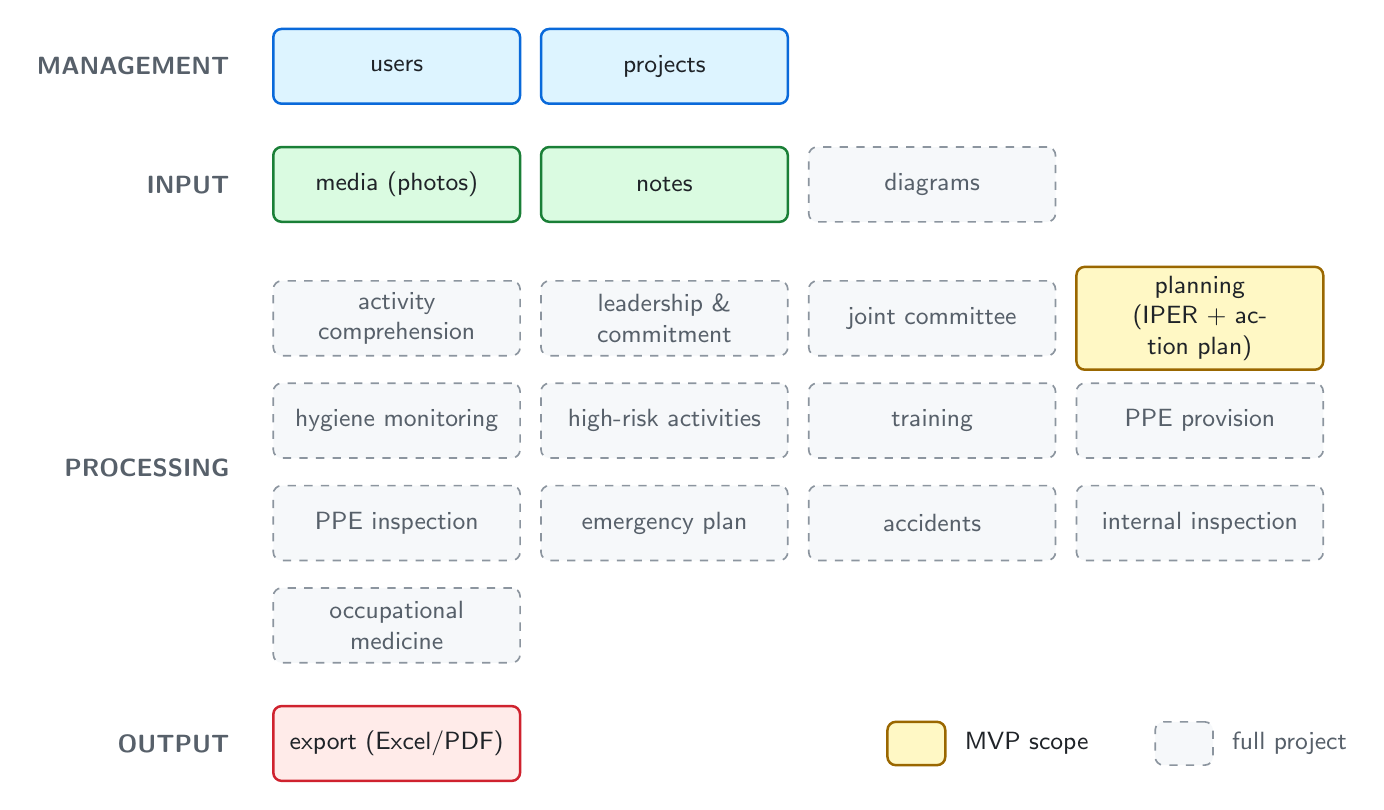
\begin{tikzpicture}[
    font=\small,
    section/.style={text=fgMuted, font=\small\bfseries, anchor=east},
    module/.style={rectangle, rounded corners=3pt, draw, line width=0.9pt,
                   text=fgText, text centered, minimum height=0.95cm, text width=2.9cm},
    mgmt/.style={module, fill=mgmtFill, draw=mgmtLine},
    input/.style={module, fill=inFill, draw=inLine},
    proc/.style={module, fill=procFill, draw=procLine},
    output/.style={module, fill=outFill, draw=outLine},
    off/.style={module, dashed, line width=0.6pt, fill=offFill, draw=offLine, text=fgMuted},
  ]

  % Column x-positions and band y-positions
  \def\cA{0}\def\cB{3.4}\def\cC{6.8}\def\cD{10.2}

  % MANAGEMENT
  \node[section] at (-2.0, 0) {MANAGEMENT};
  \node[mgmt] at (\cA, 0) {users};
  \node[mgmt] at (\cB, 0) {projects};

  % INPUT
  \node[section] at (-2.0, -1.5) {INPUT};
  \node[input] at (\cA, -1.5) {media (photos)};
  \node[input] at (\cB, -1.5) {notes};
  \node[off]   at (\cC, -1.5) {diagrams};

  % PROCESSING (one module per NTS-009/23 technical content point)
  \node[section] at (-2.0, -5.1) {PROCESSING};
  \node[off]  at (\cA, -3.2) {activity\\ comprehension};
  \node[off]  at (\cB, -3.2) {leadership \& commitment};
  \node[off]  at (\cC, -3.2) {joint committee};
  \node[proc] at (\cD, -3.2) {planning\\ (IPER + action plan)};
  \node[off]  at (\cA, -4.5) {hygiene monitoring};
  \node[off]  at (\cB, -4.5) {high-risk activities};
  \node[off]  at (\cC, -4.5) {training};
  \node[off]  at (\cD, -4.5) {PPE provision};
  \node[off]  at (\cA, -5.8) {PPE inspection};
  \node[off]  at (\cB, -5.8) {emergency plan};
  \node[off]  at (\cC, -5.8) {accidents};
  \node[off]  at (\cD, -5.8) {internal inspection};
  \node[off]  at (\cA, -7.1) {occupational medicine};

  % OUTPUT
  \node[section] at (-2.0, -8.6) {OUTPUT};
  \node[output] at (\cA, -8.6) {export (Excel/PDF)};

  % LEGEND
  \node[proc, minimum height=0.55cm, text width=0.5cm] (legmvp) at (\cC - 0.2, -8.6) {};
  \node[anchor=west, text=fgText] at (legmvp.east) {\ MVP scope};
  \node[off, minimum height=0.55cm, text width=0.5cm] (legoff) at (\cD - 0.2, -8.6) {};
  \node[anchor=west, text=fgMuted] at (legoff.east) {\ full project};

\end{tikzpicture}
\end{document}
"
%   pdftocairo -png -transp -singlefile -r 200 architecture-light.pdf architecture-light
%   pdftocairo -png -transp -singlefile -r 200 architecture-dark.pdf architecture-dark
\documentclass[tikz,border=14pt]{standalone}
\usepackage[T1]{fontenc}
\usepackage{helvet}
\renewcommand{\familydefault}{\sfdefault}
\usetikzlibrary{positioning}

\ifdefined\DARKMODE
  % GitHub dark palette
  \definecolor{fgText}{HTML}{E6EDF3}
  \definecolor{fgMuted}{HTML}{9198A1}
  \definecolor{mgmtFill}{HTML}{0D2540}\definecolor{mgmtLine}{HTML}{4493F8}
  \definecolor{inFill}{HTML}{12261E}\definecolor{inLine}{HTML}{3FB950}
  \definecolor{procFill}{HTML}{2E2A14}\definecolor{procLine}{HTML}{D29922}
  \definecolor{outFill}{HTML}{2D1418}\definecolor{outLine}{HTML}{F85149}
  \definecolor{offFill}{HTML}{161B22}\definecolor{offLine}{HTML}{545D68}
\else
  % GitHub light palette
  \definecolor{fgText}{HTML}{1F2328}
  \definecolor{fgMuted}{HTML}{57606A}
  \definecolor{mgmtFill}{HTML}{DDF4FF}\definecolor{mgmtLine}{HTML}{0969DA}
  \definecolor{inFill}{HTML}{DAFBE1}\definecolor{inLine}{HTML}{1A7F37}
  \definecolor{procFill}{HTML}{FFF8C5}\definecolor{procLine}{HTML}{9A6700}
  \definecolor{outFill}{HTML}{FFEBE9}\definecolor{outLine}{HTML}{CF222E}
  \definecolor{offFill}{HTML}{F6F8FA}\definecolor{offLine}{HTML}{8C959F}
\fi

\begin{document}
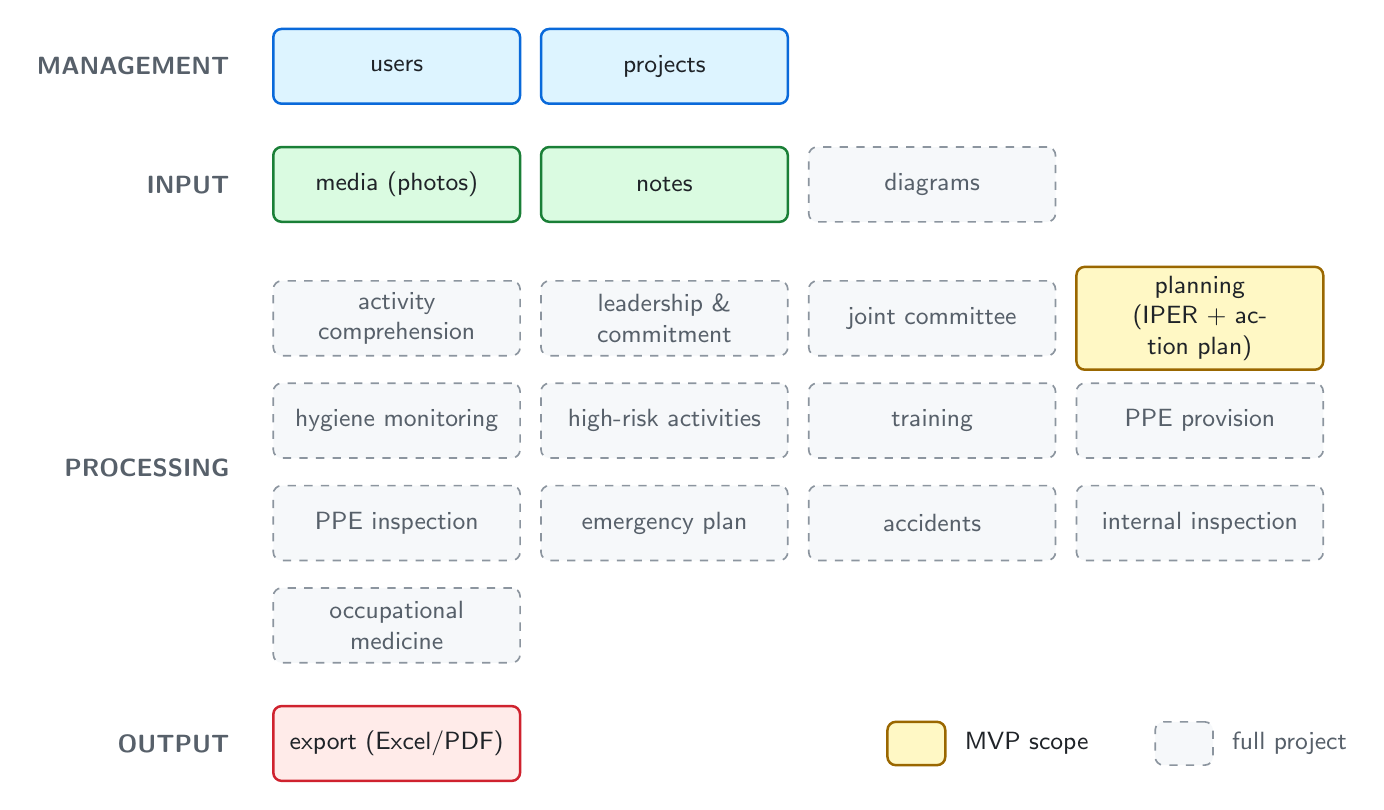
\begin{tikzpicture}[
    font=\small,
    section/.style={text=fgMuted, font=\small\bfseries, anchor=east},
    module/.style={rectangle, rounded corners=3pt, draw, line width=0.9pt,
                   text=fgText, text centered, minimum height=0.95cm, text width=2.9cm},
    mgmt/.style={module, fill=mgmtFill, draw=mgmtLine},
    input/.style={module, fill=inFill, draw=inLine},
    proc/.style={module, fill=procFill, draw=procLine},
    output/.style={module, fill=outFill, draw=outLine},
    off/.style={module, dashed, line width=0.6pt, fill=offFill, draw=offLine, text=fgMuted},
  ]

  % Column x-positions and band y-positions
  \def\cA{0}\def\cB{3.4}\def\cC{6.8}\def\cD{10.2}

  % MANAGEMENT
  \node[section] at (-2.0, 0) {MANAGEMENT};
  \node[mgmt] at (\cA, 0) {users};
  \node[mgmt] at (\cB, 0) {projects};

  % INPUT
  \node[section] at (-2.0, -1.5) {INPUT};
  \node[input] at (\cA, -1.5) {media (photos)};
  \node[input] at (\cB, -1.5) {notes};
  \node[off]   at (\cC, -1.5) {diagrams};

  % PROCESSING (one module per NTS-009/23 technical content point)
  \node[section] at (-2.0, -5.1) {PROCESSING};
  \node[off]  at (\cA, -3.2) {activity\\ comprehension};
  \node[off]  at (\cB, -3.2) {leadership \& commitment};
  \node[off]  at (\cC, -3.2) {joint committee};
  \node[proc] at (\cD, -3.2) {planning\\ (IPER + action plan)};
  \node[off]  at (\cA, -4.5) {hygiene monitoring};
  \node[off]  at (\cB, -4.5) {high-risk activities};
  \node[off]  at (\cC, -4.5) {training};
  \node[off]  at (\cD, -4.5) {PPE provision};
  \node[off]  at (\cA, -5.8) {PPE inspection};
  \node[off]  at (\cB, -5.8) {emergency plan};
  \node[off]  at (\cC, -5.8) {accidents};
  \node[off]  at (\cD, -5.8) {internal inspection};
  \node[off]  at (\cA, -7.1) {occupational medicine};

  % OUTPUT
  \node[section] at (-2.0, -8.6) {OUTPUT};
  \node[output] at (\cA, -8.6) {export (Excel/PDF)};

  % LEGEND
  \node[proc, minimum height=0.55cm, text width=0.5cm] (legmvp) at (\cC - 0.2, -8.6) {};
  \node[anchor=west, text=fgText] at (legmvp.east) {\ MVP scope};
  \node[off, minimum height=0.55cm, text width=0.5cm] (legoff) at (\cD - 0.2, -8.6) {};
  \node[anchor=west, text=fgMuted] at (legoff.east) {\ full project};

\end{tikzpicture}
\end{document}
"
%   pdftocairo -png -transp -singlefile -r 200 architecture-light.pdf architecture-light
%   pdftocairo -png -transp -singlefile -r 200 architecture-dark.pdf architecture-dark
\documentclass[tikz,border=14pt]{standalone}
\usepackage[T1]{fontenc}
\usepackage{helvet}
\renewcommand{\familydefault}{\sfdefault}
\usetikzlibrary{positioning}

\ifdefined\DARKMODE
  % GitHub dark palette
  \definecolor{fgText}{HTML}{E6EDF3}
  \definecolor{fgMuted}{HTML}{9198A1}
  \definecolor{mgmtFill}{HTML}{0D2540}\definecolor{mgmtLine}{HTML}{4493F8}
  \definecolor{inFill}{HTML}{12261E}\definecolor{inLine}{HTML}{3FB950}
  \definecolor{procFill}{HTML}{2E2A14}\definecolor{procLine}{HTML}{D29922}
  \definecolor{outFill}{HTML}{2D1418}\definecolor{outLine}{HTML}{F85149}
  \definecolor{offFill}{HTML}{161B22}\definecolor{offLine}{HTML}{545D68}
\else
  % GitHub light palette
  \definecolor{fgText}{HTML}{1F2328}
  \definecolor{fgMuted}{HTML}{57606A}
  \definecolor{mgmtFill}{HTML}{DDF4FF}\definecolor{mgmtLine}{HTML}{0969DA}
  \definecolor{inFill}{HTML}{DAFBE1}\definecolor{inLine}{HTML}{1A7F37}
  \definecolor{procFill}{HTML}{FFF8C5}\definecolor{procLine}{HTML}{9A6700}
  \definecolor{outFill}{HTML}{FFEBE9}\definecolor{outLine}{HTML}{CF222E}
  \definecolor{offFill}{HTML}{F6F8FA}\definecolor{offLine}{HTML}{8C959F}
\fi

\begin{document}
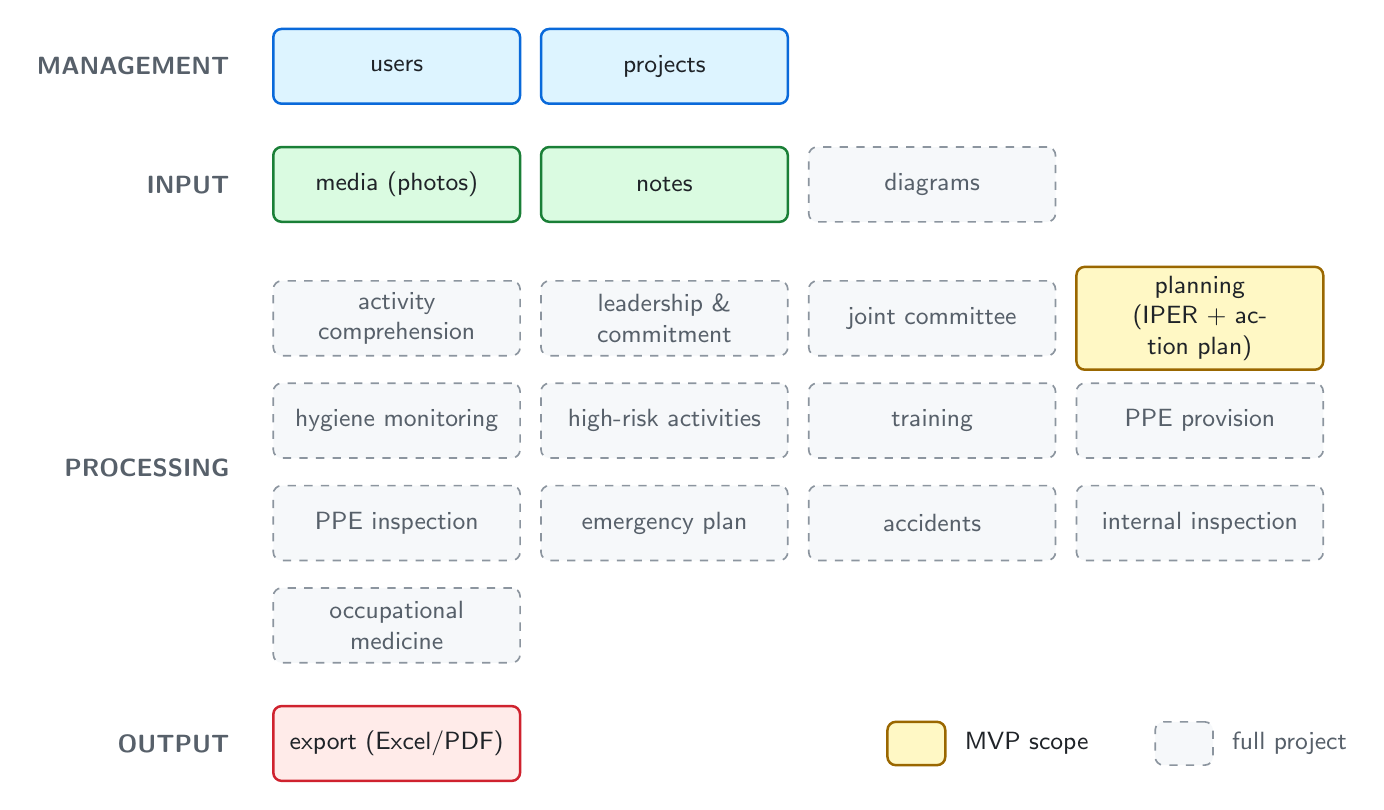
\begin{tikzpicture}[
    font=\small,
    section/.style={text=fgMuted, font=\small\bfseries, anchor=east},
    module/.style={rectangle, rounded corners=3pt, draw, line width=0.9pt,
                   text=fgText, text centered, minimum height=0.95cm, text width=2.9cm},
    mgmt/.style={module, fill=mgmtFill, draw=mgmtLine},
    input/.style={module, fill=inFill, draw=inLine},
    proc/.style={module, fill=procFill, draw=procLine},
    output/.style={module, fill=outFill, draw=outLine},
    off/.style={module, dashed, line width=0.6pt, fill=offFill, draw=offLine, text=fgMuted},
  ]

  % Column x-positions and band y-positions
  \def\cA{0}\def\cB{3.4}\def\cC{6.8}\def\cD{10.2}

  % MANAGEMENT
  \node[section] at (-2.0, 0) {MANAGEMENT};
  \node[mgmt] at (\cA, 0) {users};
  \node[mgmt] at (\cB, 0) {projects};

  % INPUT
  \node[section] at (-2.0, -1.5) {INPUT};
  \node[input] at (\cA, -1.5) {media (photos)};
  \node[input] at (\cB, -1.5) {notes};
  \node[off]   at (\cC, -1.5) {diagrams};

  % PROCESSING (one module per NTS-009/23 technical content point)
  \node[section] at (-2.0, -5.1) {PROCESSING};
  \node[off]  at (\cA, -3.2) {activity\\ comprehension};
  \node[off]  at (\cB, -3.2) {leadership \& commitment};
  \node[off]  at (\cC, -3.2) {joint committee};
  \node[proc] at (\cD, -3.2) {planning\\ (IPER + action plan)};
  \node[off]  at (\cA, -4.5) {hygiene monitoring};
  \node[off]  at (\cB, -4.5) {high-risk activities};
  \node[off]  at (\cC, -4.5) {training};
  \node[off]  at (\cD, -4.5) {PPE provision};
  \node[off]  at (\cA, -5.8) {PPE inspection};
  \node[off]  at (\cB, -5.8) {emergency plan};
  \node[off]  at (\cC, -5.8) {accidents};
  \node[off]  at (\cD, -5.8) {internal inspection};
  \node[off]  at (\cA, -7.1) {occupational medicine};

  % OUTPUT
  \node[section] at (-2.0, -8.6) {OUTPUT};
  \node[output] at (\cA, -8.6) {export (Excel/PDF)};

  % LEGEND
  \node[proc, minimum height=0.55cm, text width=0.5cm] (legmvp) at (\cC - 0.2, -8.6) {};
  \node[anchor=west, text=fgText] at (legmvp.east) {\ MVP scope};
  \node[off, minimum height=0.55cm, text width=0.5cm] (legoff) at (\cD - 0.2, -8.6) {};
  \node[anchor=west, text=fgMuted] at (legoff.east) {\ full project};

\end{tikzpicture}
\end{document}
"
%   pdftocairo -png -transp -singlefile -r 200 architecture-light.pdf architecture-light
%   pdftocairo -png -transp -singlefile -r 200 architecture-dark.pdf architecture-dark
\documentclass[tikz,border=14pt]{standalone}
\usepackage[T1]{fontenc}
\usepackage{helvet}
\renewcommand{\familydefault}{\sfdefault}
\usetikzlibrary{positioning}

\ifdefined\DARKMODE
  % GitHub dark palette
  \definecolor{fgText}{HTML}{E6EDF3}
  \definecolor{fgMuted}{HTML}{9198A1}
  \definecolor{mgmtFill}{HTML}{0D2540}\definecolor{mgmtLine}{HTML}{4493F8}
  \definecolor{inFill}{HTML}{12261E}\definecolor{inLine}{HTML}{3FB950}
  \definecolor{procFill}{HTML}{2E2A14}\definecolor{procLine}{HTML}{D29922}
  \definecolor{outFill}{HTML}{2D1418}\definecolor{outLine}{HTML}{F85149}
  \definecolor{offFill}{HTML}{161B22}\definecolor{offLine}{HTML}{545D68}
\else
  % GitHub light palette
  \definecolor{fgText}{HTML}{1F2328}
  \definecolor{fgMuted}{HTML}{57606A}
  \definecolor{mgmtFill}{HTML}{DDF4FF}\definecolor{mgmtLine}{HTML}{0969DA}
  \definecolor{inFill}{HTML}{DAFBE1}\definecolor{inLine}{HTML}{1A7F37}
  \definecolor{procFill}{HTML}{FFF8C5}\definecolor{procLine}{HTML}{9A6700}
  \definecolor{outFill}{HTML}{FFEBE9}\definecolor{outLine}{HTML}{CF222E}
  \definecolor{offFill}{HTML}{F6F8FA}\definecolor{offLine}{HTML}{8C959F}
\fi

\begin{document}
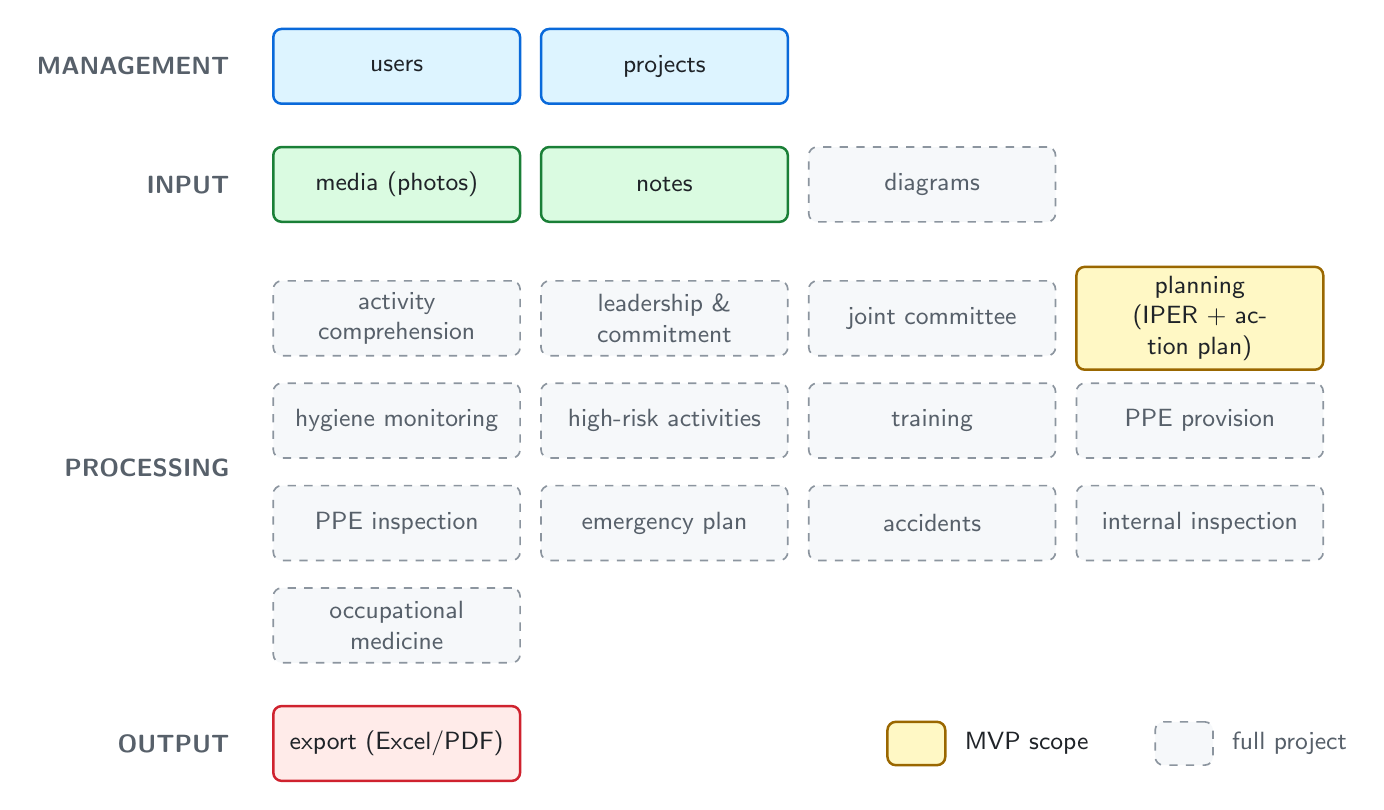
\begin{tikzpicture}[
    font=\small,
    section/.style={text=fgMuted, font=\small\bfseries, anchor=east},
    module/.style={rectangle, rounded corners=3pt, draw, line width=0.9pt,
                   text=fgText, text centered, minimum height=0.95cm, text width=2.9cm},
    mgmt/.style={module, fill=mgmtFill, draw=mgmtLine},
    input/.style={module, fill=inFill, draw=inLine},
    proc/.style={module, fill=procFill, draw=procLine},
    output/.style={module, fill=outFill, draw=outLine},
    off/.style={module, dashed, line width=0.6pt, fill=offFill, draw=offLine, text=fgMuted},
  ]

  % Column x-positions and band y-positions
  \def\cA{0}\def\cB{3.4}\def\cC{6.8}\def\cD{10.2}

  % MANAGEMENT
  \node[section] at (-2.0, 0) {MANAGEMENT};
  \node[mgmt] at (\cA, 0) {users};
  \node[mgmt] at (\cB, 0) {projects};

  % INPUT
  \node[section] at (-2.0, -1.5) {INPUT};
  \node[input] at (\cA, -1.5) {media (photos)};
  \node[input] at (\cB, -1.5) {notes};
  \node[off]   at (\cC, -1.5) {diagrams};

  % PROCESSING (one module per NTS-009/23 technical content point)
  \node[section] at (-2.0, -5.1) {PROCESSING};
  \node[off]  at (\cA, -3.2) {activity\\ comprehension};
  \node[off]  at (\cB, -3.2) {leadership \& commitment};
  \node[off]  at (\cC, -3.2) {joint committee};
  \node[proc] at (\cD, -3.2) {planning\\ (IPER + action plan)};
  \node[off]  at (\cA, -4.5) {hygiene monitoring};
  \node[off]  at (\cB, -4.5) {high-risk activities};
  \node[off]  at (\cC, -4.5) {training};
  \node[off]  at (\cD, -4.5) {PPE provision};
  \node[off]  at (\cA, -5.8) {PPE inspection};
  \node[off]  at (\cB, -5.8) {emergency plan};
  \node[off]  at (\cC, -5.8) {accidents};
  \node[off]  at (\cD, -5.8) {internal inspection};
  \node[off]  at (\cA, -7.1) {occupational medicine};

  % OUTPUT
  \node[section] at (-2.0, -8.6) {OUTPUT};
  \node[output] at (\cA, -8.6) {export (Excel/PDF)};

  % LEGEND
  \node[proc, minimum height=0.55cm, text width=0.5cm] (legmvp) at (\cC - 0.2, -8.6) {};
  \node[anchor=west, text=fgText] at (legmvp.east) {\ MVP scope};
  \node[off, minimum height=0.55cm, text width=0.5cm] (legoff) at (\cD - 0.2, -8.6) {};
  \node[anchor=west, text=fgMuted] at (legoff.east) {\ full project};

\end{tikzpicture}
\end{document}
